\documentclass[letterpaper,twocolumn,12pt]{article}
\usepackage{usenix-2020-09}
\usepackage{tikz}
\usepackage{amsmath}
\usepackage{hyperref}
\usepackage{listings}
\lstset{
	basicstyle=\small,
	columns=fullflexible,
	frame=single,
	breaklines=true,
	language=C++,
	captionpos=b,
	numbers=left,
	belowskip=-0.1 \baselineskip,
	commentstyle=\color{blue},
	postbreak=\mbox{\textcolor{red}{$\hookrightarrow$}\space}
}
\hyphenation{Complexity-wise}

%-------------------------------------------------------------------------------
\begin{document}
%-------------------------------------------------------------------------------

%don't want date printed
\date{}

\title{\Large \bf Towards the Design of CANLay: A User-centered Overlay for In-Vehicle Data Dissemination In a Network Virtualized Testbed}

% %for single author (just remove % characters)
% \author{
% {\rm Jacob Jepson}\\
% Colorado State University
% \and
% {\rm Subhojeet Mukherjee}\\
% Colorado State University
% % copy the following lines to add more authors
% \and
% {\rm Jeremy Daily}\\
% Colorado State University
% } % end author

\maketitle

%-------------------------------------------------------------------------------
\begin{abstract}
%-------------------------------------------------------------------------------
This paper presents the design of CANLay, the networking backbone of the Software Defined Truck \cite{mukherjee_towards_2021}, a network virtualized testbed for in-vehicle network security testing. CANLay, is responsible for carrying controller area network data as well as sensor signals emanating from the vehicle. As such, CANLay acts as a communication media between a vehicle simulator and real-world electronic control units located on different network segments. Towards the end of the paper, we present a discussion on CANLay's appication in a real-world usage scnerio.
\end{abstract}

\section{Introduction and Background}
%-------------------------------------------------------------------------------
In recent years security of the Controller Area Network (CAN) has been a much talked about topic of research. CAN is a broadcast media that enables reliable and low-latency communication between in-vehicle devices, also referred to as Electronic Control Units (ECU). This broadcast nature of CAN, along with the fact that it is inherently unauthenticated, makes it susceptible to network-wide cyber threats. 
Security researchers have shown \cite{checkoway_comprehensive_2011, mukherjee_practical_2016,burakova_truck_2016} that remote interfaces on modern vehicles can be used to intrude into internal CAN networks and inject messages to control and/or disrupt the operations of the vehicle. At the same time, the development of security solutions can be pursued to detect and/or prevent this scenario from occurring.

To evaluate the effectiveness of their proposed techniques, researchers have typically experimented on real-vehicles or homegrown testbed setups that mimic real vehicles. 
While most households in the United States have at least one passenger car \cite{mathilde_carlier_number_2021}, this is not the same for medium and heavy-duty (MHD) vehicles. 
Moreover, creating homegrown testbeds is both logistically and economically challenging. To that end, the need for a publicly accessible testbench is imminent. This is where the concept of the Software Define Truck (SDT) \cite{mukherjee_towards_2021} is critical to the in-vehicle networking community. It aims to provide a distributed network virtualized platform on which in-vehicle security experiments can be performed. Although proposed primarily for the heavy-trucks, SDT can easily be adapted for lightweight passenger vehicles. SDT's information exchange goal is shown in figure \ref{fig:goal}. CAN frames and physical signals need to be exchanged between ECUs and vehicle simulators located in different subnetworks around the globe. CANLay is the networking backbone of the SDT and aims to provide the necessary infrastructure to enable this service.

\begin{figure}[]
    \centering
    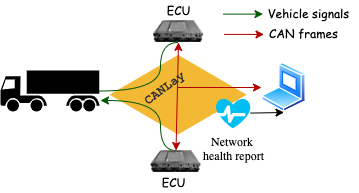
\includegraphics[width=\linewidth]{images/design_goal.drawio.png}
    \caption{Purpose of CANLay}
    \label{fig:goal}
\end{figure}

Previous research \cite{tagarev_automotive_2021} has established two critical criteria for quality evaluation of automotive networking testbeds: fidelity and adaptability. Fidelity is the ability to emulate a real-world in-vehicle networking infrastructure. Adaptability is the ability to simulate different real-world in-vehicle networking infrastructures. 
% As such, it may be difficult to optimize both. An adaptable system requires virtualized components that adjust quickly to suit users' needs. 
As such, it may be challenging to optimize both. An adaptable system requires virtualized components that adjust quickly to suit users' needs. 
% To make a system adaptable, the underlying components need to be virtualized so they can be reconfigured to suit user needs. 
Albeit, this hampers the fidelity of the system. While CANLay provides the means to configure experiment networks on-demand, it also provides a real-time health report for the underlying network. 
This feature allows the user to assess the fidelity of the overlay in terms of standard networking metrics like latency, rate of packet drop, etc.
% This allows the user to assess the fidelity of the overlay in terms of standard networking metrics like latency, rate of packet drop, etc.

Although CAN is a relatively new communication technology and has a smaller application scope than TCP/IP, there have been some proposals to virtualize its operations. 
First, there has been the attempt to adapt the software-defined networking paradigm for CAN \cite{rotermund_requirements_2020,doering_retrofitting_nodate,grewe_bloomycan_2021}. This approach is largely hardware-based and is catered for in-vehicle networking on CAN physical channels, not over long-range overlays. For range relaying of CAN frames, there has been the CAN-to-ethernet direction of research \cite{johanson_relaying_2009,florian_polzlbauer_experience_2019}. 
The goal is not to enable ECU-to-ECU communication rather transportation of data logged from one network to a remote endpoint. 
% The goal is not to enable ECU-to-ECU communication, rather transportation of data logged from one network to a remote endpoint. 
Configurability and network performance are usually not addressed. Neither is the CAN-to-ethernet paradigm designed to transport physical signals over long distances. 
X-in-the-loop (hardware, driver, vehicle, etc.) simulation-based in-vehicle testbeds \cite{appel_safety_2020} have been proposed, but the signals from the simulators have been transported over physical connections, not over reconfigurable, long-range network overlays. 

At this time, CANLay has the following functional objectives:
\begin{itemize}
    \item Transport of CAN frames over a distributed overlay network of electronic control units
    \item Transport of sensor signals to a distributed network of electronic control units
    \item Supporting the creation of these overlays on-demand
    \item Provision of runtime metrics to estimate the network health during the ongoing experiment.
    % \item Provision of runtime metrics to estimate the health of the network during the ongoing experiment.
\end{itemize}
In the rest of this paper, we describe the design of CANLay (section \ref{sec:design}), provide a discussion on its usage in an example scenario (\ref{sec:usage}), and finish with conclusive remarks and future works.

\section{Design and Current Development}\label{sec:design}
\begin{figure*}[]
    \centering
    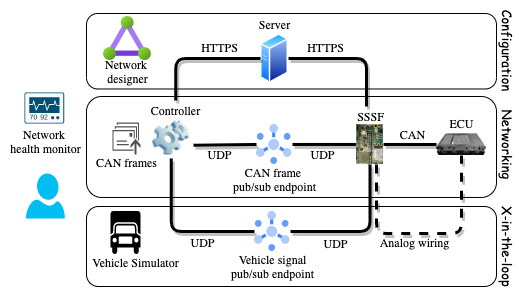
\includegraphics[width=\linewidth]{images/system_design.drawio.png}
    \caption{Proposed System}
    \label{fig:system}
\end{figure*}
Figure \ref{fig:system} shows the proposed system design of CANLay. The system serves three functions: offline configuration of the network overlay and CAN frame and vehicle signal exchange at runtime. 
Next, we will describe the components and their roles in the system. 
% A description of the components and their roles in the system is provided next. 
Following that, we will describe the behavioral aspects of the system. 
% Following that, a description of the behavioral aspects of the system is provided. 
Together, these aspects combine to accomplish the functional objectives.

% ECUs in our system are required to interface with Smart sensors Simulator (SSSF) devices. These devices act as gateways to the CANLay system. At startup they communicate with a central Server thereby registering themselves. This communication happens over HTTP(s). 

% \subsection{Current Status of Development}

\subsection{Component Descriptions}
\subsubsection{Smart sensor Simulator and Forwarder (SSSF)}
The Smart Sensor Simulator and Forwarder acts as a gateway enabling the ECU to access and to be accessed by the CANLay system. 
In an active experiment, the SSSF acts as a forwarder between the Controller and the ECU through User datagram protocol (UDP) channels and CAN interfaces. SSSFs can forward two types of messages. 
% In an active experiment, it acts as a forwarder between the Controller and the ECU through User datagram protocol (UDP) channels and CAN interfaces. SSSFs can forward two types of messages. 
The first type carries signals from the vehicle simulator. Eventually, these signals may have to transmit along the analog wiring shown using a dashed line figure \ref{fig:system}.  
The second type is CAN data carried from the ECUs in the current experiment. Through the SSSFs, multiple ECUs can communicate with each other to create a rich testing environment.
% The second type is CAN data carried from the ECUs as well as from other SSSFs in the current experiment. Through the SSSFs, multiple ECUs can actively communicate with each other to create a rich testing environment.

The SSSF is developed a built on a Teesny 3.6 .... a paragraph describing the SSS2's. Talk about SD cards. PLease include a block diagram etc.
CAN Forwarding 
%TODO Dr. Daily can help
The real-time clock on the SSF is synchronized through the network time protocol (NTP).

\subsubsection{Controller}
The Controller is the user's interface to the CANLay system and enables vehicle simulators to communicate with the CANLay network. The Controller User Interface (UI) is used to assist the user in building their virtual testbed. 
It does so by communicating with the central Server over hypertext transfer protocol secure (HTTPS). 
Once the experiment setup finishes, the Controller transitions to acting as a gateway for a graphical vehicle simulator to communicate with the CANLay system by forwarding the simulator's outputs to the publish/subscribe (pub/sub) endpoint and listening for CAN messages from the same.
% Once the experiment setup finishes, the Controller transitions to acting as a gateway for a graphical vehicle simulator to communicate with the CANLay system. It forwards simulator outputs to the publish/subscribe (pub/sub) endpoint and listens for CAN messages from the same.

The Controller is a multithreaded graphical application built using python. It exposes two UI components, namely, the Network Designer and the Network Health Monitor. 
The Controller manages the execution of the Vehicle Simulator to ensure that it stays "in-step" with the flow of signals produced. 
% The Controller manages the execution of the Vehicle Simulator ensuring that it stays "in-step" with the flow of signals being produced. 
In addition, the Controller is in charge of updating the Network Designer's catalog of available devices and relaying the virtual network designs of the user to the Server. The Controller efficiently manages the multiple streams of incoming and outgoing data using Selectors. Selectors enable the Controller to know when a socket is available to read or write. Finally, once a session has begun, the Controller manages the aggregation and presentation of network health reports. The Controller collects the current statistics from all devices in the session and displays the results using heat matrices. Further discussion of the heat matrices occurs later in the paper.

\subsubsection{Server}
The Server helps in setting up the publishers and subscribers for an experiment. Each device opens and maintains a persistent transmission control protocol (TCP) connection with the Server while participating in the CANLay system. 
After establishing the TCP connection, the devices communicate with the Server through HTTP application programming interfaces (API). 
% Once the TCP connection is established the devices communicate with the Server through HTTP application programming interfaces (API). 
The Server can monitor the health of the devices and take action if a device is malfunctioning or goes offline. 
This mechanism also allows the Server to keep track of free SSSFs and pub/sub endpoints to validate new experiment requests and allocate the requested devices and endpoints. This technique avoids the race conditions or double use issues that may arise if each Controller was in charge of gathering the requested SSSFs for its experiment. 
% This mechanism also allows the Server to keep track of free SSSFs and free pub/sub endpoints, so it can validate new experiment requests and allocate the requested devices and endpoints without running into race conditions or double use issues that may arise if each Controller was in charge of allocating its own experiment. 
Finally, the Server keeps track of ongoing sessions and ensures the proper closure of sessions when a device is experiencing issues.
% Finally, the Server keeps track of ongoing experiments and ensures the proper closure of an experiment in the event a device is experiencing issues.

The Server is a single-threaded session broker that multiplexes the handling of HTTP API calls using Selectors. 
% The Server is a single-threaded session broker that multiplexes the handling of HTTP API calls through the use of Selectors. 
We chose HTTP API calls because they clearly define the target object to invoke and how to invoke it. The devices perform all necessary setup and teardown actions such as registering, deregistering, starting and stopping a session by sending HTTP requests to different API endpoints. 
The Server responds to these requests using standard HTTP response messages and codes that are easily interpretable by both the devices and users.
% The Server responds to these requests using standard HTTP response messages and codes which can be easily interpreted by both the devices and users.

\subsubsection{Publish/Subscribe Endpoints}
UDP is used to connect the publishers and subscribers in the CANLay system. 
% A pub/sub endpoint in the CANLay network is a pub/sub address and port pair. Although the CAN frame and Vehicle signal pub/sub endpoints are shown separately in the above diagram for clarity, they are physically a single endpoint in the network. 
We chose the pub/sub model because it can easily emulate the broadcast nature of CAN \cite{kaiser_implementing_1999} in that an ECU is subscribed to all other ECUs on the same CAN bus, and all other ECUs on that CAN bus are subscribed to that ECU. 

We used two criteria to find a suitable pub/sub mechanism that resembles a CAN network. 
% To find a suitable pub/sub mechanism that closely resembles a CAN network, we used two criteria. 
First, the transport mechanism must support some form of message broadcasting that enables a sender to send one message that can be received by many receivers; without significant duplication and delay-related overheads \cite{kaiser_implementing_1999}. 
The first is that the transport mechanism must support some form of message broadcasting that enables a sender to send one message that can be received by many receivers without significant duplication and delay-related overheads \cite{kaiser_implementing_1999}. 
Next, the transport mechanism must permit the devices to receive messages from one or more devices while maintaining only one connection.

At this time, we have chosen UDP multicasting as a suitable pub/sub mechanism as it does not require a message broker with high-performance requirements. We realize that multicasting outside a local network may lead to increased costs for the implementers, but the current goal was to test its usability and make future decisions based on the observed performance. At this time, we are also exploring other potential pub/sub implementations such as MQTT.

\subsubsection{Front-End Components}
\begin{figure}[]
    \centering
    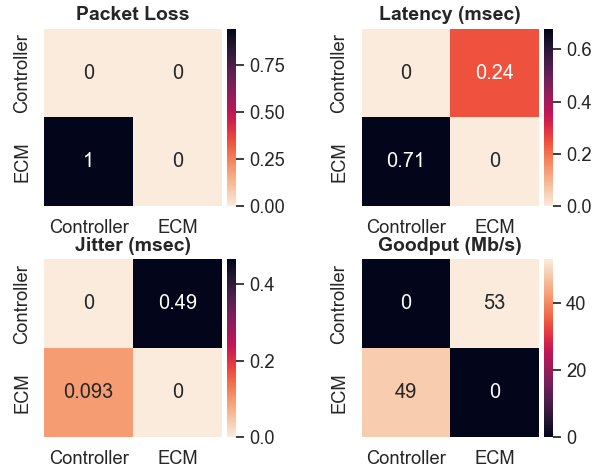
\includegraphics[width=\linewidth]{images/network_matrix.png}
    \caption[]{Network Matrices showing packet loss, latency, jitter, and goodput.}
    \label{fig:network_matrix}
\end{figure}
\begin{figure*}[]
    \centering
    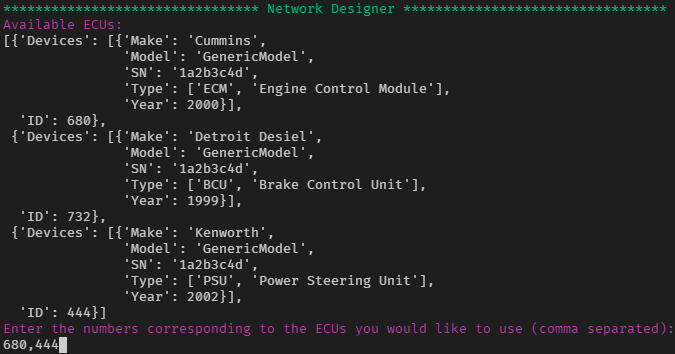
\includegraphics[width=\linewidth]{images/network_designer.png}
    \caption[]{Network Designer displaying available ECUs\protect\footnotemark}
    \label{fig:network_designer}
\end{figure*}

As seen in figure \ref{fig:network_designer}, the Network Designer consists of a catalog of available devices and the ability to select the requested devices. Upon startup, the Controller contacts the Server and solicits the set of available devices. The Controller then presents these options to the user and allows them to select the requested devices from the catalog of available ECUs.

\footnotetext{Currently, the network designer is controlled through the command line but in the future, a GUI will be added that performs the same function.}

As seen in figure \ref{fig:network_matrix}, the Network Health Monitor shows real-time network statistics that describe the current state of the network. These statistics are presented using heat matrices. Each cell in the matric represents a directed communication channel of the network. The color of the cells depends on their values. For packet loss, latency, and jitter (significance and method of evaluation for these metrics are described later) the lower the number the better and the lighter the color will be. For goodput, the higher the number the better and the lighter the color will be. The contrast between the light and dark colors allows the user to quickly spot the underperforming parts of the network.

\subsection{Behavior Descriptions}

\subsubsection{Network Setup (ref. figure \ref{fig:setup_activity})}
\begin{figure*}[]
    \centering
    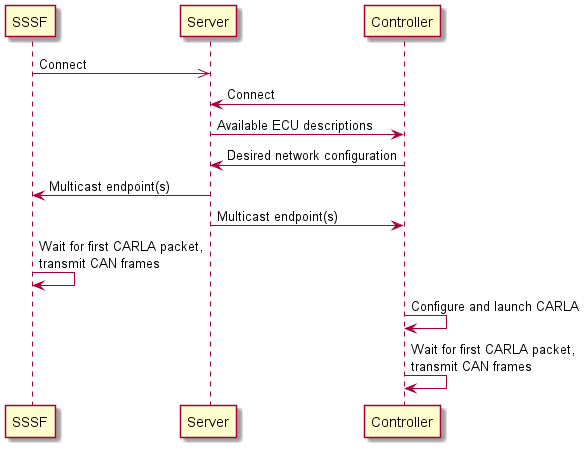
\includegraphics[scale=0.8]{out/images/connection_setup/connection_setup.png}
    \caption{Network Setup Activity}
    \label{fig:setup_activity}
\end{figure*}
While the Server is up and running, SSSFs connect to it. SSSFs perform a setup procedure by reading their inbuilt SD card. The type, year, make, model, and the serial number of the connected ECUs are read from a predefined file stored on the SD card. Next, the SSSF gathers its MAC address and list of attached devices into a JSON and sends it to the Server via a POST to the HTTP API endpoint /\textit{SSSF}/\textit{Register}. 
If the registration fails, the Server responds with an HTTP 4XX error code indicating why the registration was unsuccessful. Otherwise, the Server responds with an HTTP 202 code indicating the SSSF was accepted. Once successfully registered, the SSSF waits for further instructions from the Server on its HTTPS port. 

The Controller begins by registering with the Server similarly to the SSSF, except that the Controller has no attached devices, so it only sends its MAC address to the Server.
Once successfully registered, the Controller requests a list of the available{\footnote{If an SSSF device is currently being used in another experiment it is not considered available.}} ECUs. After receiving the list of available devices, it presents the available ECUs to the user via the Network Designer described earlier. Notice that while the Server deals with SSSFs, a user will typically only be interested in the ECUs that the SSSF is acting as a gateway for. After the user finalizes their selection, the Controller sends the selected devices to the Server via an HTTP POST and waits for the Server's reply.

The Server receives the list of requested devices and performs three checks. First, it checks that the request is coming from a registered Controller. Controllers are the only devices allowed to start sessions. Next, the Server double-checks that the devices are still available. If any of the devices are no longer available or become unavailable during the setup process, the Server responds to the Controller with the error code 409, indicating a conflict in the selection. If all the devices are still available, the Server then selects a vacant pub/sub endpoint for the experiment and assigns an index to each device. The index aids the collection of network statistics which is explained later on. Now the Server sends the connection data to the Controller and SSSFs. Connection data contains a unique identifier (ID), the index, 
% of the device 
% that identifies the position of the recipient in the list of networked devices, 
a multicast IP address and port acting as the pub/sub endpoint, and a list containing the IDs and attached devices of other nodes in the experiment.

Once endpoints receive the connection data, they resync with NTP, allocate space for the required data structures, and begin listening for and forwarding messages to and from the pub/sub endpoint. At this point, the experiment setup is completed.

% \begin{figure}[]
%     \centering
%     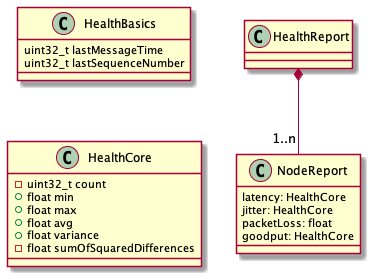
\includegraphics[width=\linewidth]{out/images/network_health/network_health.png}
%     \caption{}
%     \label{fig:}
% \end{figure}
\begin{figure}[]
    \centering
    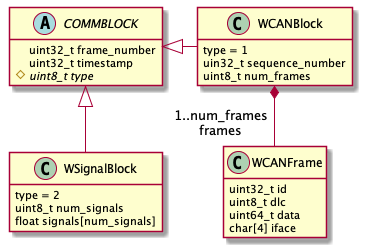
\includegraphics[width=\linewidth]{out/images/data_structures/data_structures.png}
    \caption{Transport Data Structures}
    \label{fig:ds}
\end{figure}

\begin{figure*}[]
    \centering
    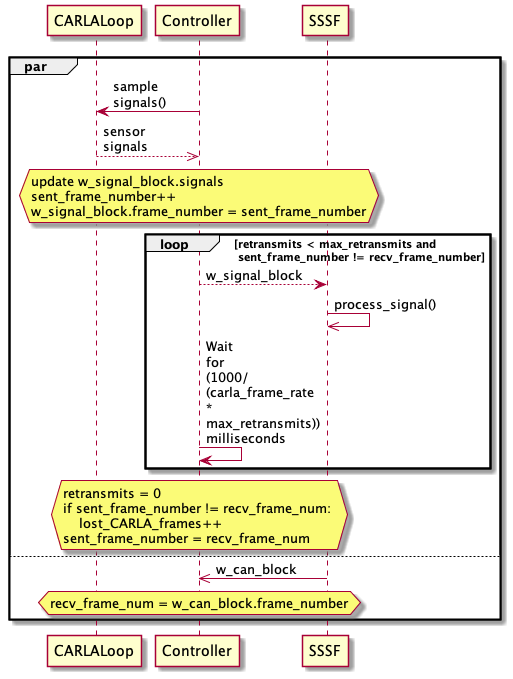
\includegraphics[scale=0.8]{out/images/signal_control/signal_control.png}
    \caption{Signal Tranmission Activity}
    \label{fig:sig_x}
\end{figure*}
\subsubsection{Sensor Signal Communication (ref. figure \ref{fig:sig_x})} \label{sec:sig_x}


Once the Controller establishes an active session, it begins forwarding sensor signals to the pub/sub endpoint. Before sending out the sensor signals, the Controller wraps them in a WsensorBlock and then a COMMBlock. There are several additional pieces of information the COMMBlock requires, but we will focus on type and frame number for now. The type indicates the subclass that the COMMBlock is carrying. In this case, the type will be 2, implying that it is transporting a WsensorBlock. The frame number is added to the COMMBlock and incremented by one every time the Controller forwards a sensor message to the CANLay network. When SSSFs send out CAN messages, they will set their outgoing COMMBlock's frame number to the last received frame number from the Controller. When the Controller receives a CAN message, it'll read the frame number field and know the latest sensor message that the SSSF received. This technique creates an acknowledgment feedback loop enabling the Controller to tell which devices have received a frame and when a frame was lost. This acknowledgment feedback loop is possible because CAN messages get sent at a higher rate than the sensor message are. 
The benefit of this acknowledgment mechanism is that it does not require additional replies from the receiver.
% This enables an acknowledgment mechanism that does not require any additional messages.

Before starting the session, the Controller lets the user select the maximum number of retransmissions. This number gets factored into the timeout value of a sensor frame. 
% Before starting the session, the Controller lets the user select the maximum number of retransmissions which is then used to calculate the timeout value of a sensor frame. 
The timeout value is calculated as follows: $1/(simulator\_frame\_rate * max\_retransmitions)$. When the Controller detects that the last frame has timed out, it first checks if it has reached its maximum number of retransmissions. If not, it will resend the sensor message, increment the number of retransmissions it performed, and reset the timeout timer. It will repeat this process until it receives a CAN message with a frame number equal to the Controller's current frame number or the Controller reaches the maximum number of retransmissions. In the latter case, the frame is considered lost, and a counter \texttt{lost\_simulator\_frames} is updated to later show to the user.

As mentioned before, when an SSSF receives a sensor frame, it first sets its last seen frame number equal to the message's frame number. Next, the SSSF applies any necessary transformations to the sensor frame before forwarding it onto its device's CAN network(s). For this paper, the transformations served mainly as a proof of concept and were kept simple, often sending just the raw sensor value in with the closest matching PGN CAN frame.
%TODO update the figure.. it is not in sync with the writting in this section .e.g. you are not using the update_health for just frames

\subsubsection{CAN Communication (ref. figure \ref{fig:can_x})}
\begin{figure*}[]
    \centering
    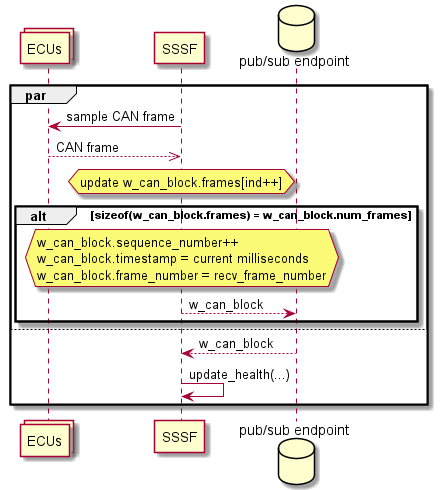
\includegraphics[scale=0.9]{out/images/can_exchange/can_exchange.png}
    \caption{CAN Communication Activity}
    \label{fig:can_x}
\end{figure*}
% In order to create the simulated CAN network of ECUs, the devices must be able to communicate with each other with minimum per
% as if they were talking via a CAN bus. 
% Most ECUs do not come with built in ethernet ports and the ability to broadcast CAN frames via Ethernet. So in order to connect an ECU to Ethernet we need a device that can interface with a CAN network and interface with an Ethernet Network. This is why 
% the Smart sensor Simulator and Forwarder is necessary. It acts as a programmable gateway that can transfer messages between the CAN network and the Ethernet Network.

When the SSSF is in an active experiment, it attempts to read a message from the CAN network. Upon doing so, it creates the COMMBlock data structure (ref. figure \ref{fig:ds}) that will get written to the CANLay network. 
% In the current scenario we set \texttt{num\_frames} to 1. Therefore, a COMMBlock data structure is transmitted after the receipt of every message.
Additional information is added to the COMMBlock before its written to the network. Several pieces of information are required, but we will focus on two right now, namely, type and sequence number.
% , and needs\_response. 
The type indicates the subclass that the COMMBlock is carrying. In this case, the type will be 1, implying that it is carrying a WCANBlock. 
The sequence number is added to the WCANBlock and incremented every time a CAN message gets sent from the device. 
% Since the message rates of sensor and CAN messages differ the acknowledgement mechanism described in the previous section works. However the sequence number included in the WCANBlock is still used for acknowledgements and 
The packet loss mechanism described later depends on this sequence number. 
% It is included to detect pack loss, a mechanism that is described later. 
% The acknowledgement mechanism for CAN messages works differently compared to the acknowledgement mechanism described before. Whereas every sensor message is implicitly acknowledged, CAN messages are explicitly acknowledged when \textit{needs\_response} is set to true. The field \textit{needs\_response} is set to true if its CAN frame’s PGN matches a list received from the user during setup.

After the SSSF finishes checking for CAN messages from the CAN network, it checks for messages from the pub/sub network.
% Again, CAN messages sent to the pub/sub endpoint are considered type 1 messages. 
% So if an SSSF device receives a type 1 message it first checks if the message requires a response. If so, it replies to the pub/sub endpoint with a type 5 message with the frame number equal to the sequence number of the message it just received. 
Upon receiving a CAN message wrapped in the \texttt{w\_can\_block}, the SSSF updates its network statistics, extracts the WCANFrame, and writes it onto its available CAN networks.

\subsubsection{Network health monitoring (ref. listings \ref{code:calc} and \ref{code:update})}\label{sec:nethealth}

\begin{lstlisting}[caption={calculate\_health(HealthCore \&networkEdge, n)}, label=code:calc, float=t]
networkEdge.min = min(networkEdge.min, n);
networkEdge.max = max(networkEdge.max, n);
networkEdge.count++;
delta = n - networkEdge.mean;
networkEdge.mean += delta / networkEdge.count;
delta2 = n - networkEdge.mean;
networkEdge.sumOfSqrdDiffs += delta * delta2;
networkEdge.variance = networkEdge.sumOfSqrdDiffs / networkEdge.count;
\end{lstlisting}

\begin{lstlisting}[caption={update\_health(ind, packetsz, ts, seq)},label=code:update, float=t] 
now = timeClient->getEpochTimeMS();
delay = now - ts;
ellapsedSeconds = (now - HealthBasics[ind].lastMessageTime);
ellapsedSeconds /= 1000.0;
calculate(HealthReport[ind].latency, abs(delay));
calculate(HealthReport[ind].jitter,HealthReport[ind].latency.variance);
pcktsLost = seq - (HealthBasics[ind].lastSequenceNumber + 1);
HealthReport[i].pcktLoss += (pcktsLost > 0) ? pcktsLost : 0;
calculate(HealthReport[ind].goodput,(packetsz * 8)/ellapsedSeconds);
HealthBasics[i].lastMessageTime = now;
HealthBasics[i].lastSequenceNumber = seq;
\end{lstlisting}

\begin{figure}[]
    \centering
    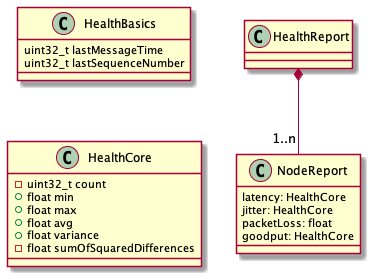
\includegraphics[width=\linewidth]{out/images/network_health/network_health.png}
    \caption{Network Health Data Structures}
    \label{fig:network_health_ds}
\end{figure}

Monitoring the health of the network is key to ensuring that unnecessary delay and packet loss are not affecting the output of the experiment. 
Each message structure from figure \ref{fig:ds} gets loaded with additional information enabling the devices to collect network statistics during an active experiment. 
% To enable the devices to collect network statistics during an active experiment, each message structure from figure \ref{fig:ds} is loaded with additional information. 
The first piece of additional information is a frame or sequence number. When other devices spot gaps in these numbers greater than 1, they know that a message was lost.
% The next important metric included in the COMMBlock messages is a timestamp. 
Next, the timestamp gets included to allow devices to calculate the latency along the network edge from the sending device to the receiving device without interrupting the testing.
% The timestamp is included to allow devices to calculate the latency along the network edge from the sending device to the receiving device.
% The timestamp is included with each message that is sent so that network health metrics can be calculated without interrupting the testing. 
The latency is calculated by subtracting the time at which the message was sent from the time at which the message was received. To ensure accuracy every device on the CANLay network implements NTP to synchronize their clocks.

These indicators enable each device to calculate four network statistics for every other device on the network. Currently, these statistics include \emph{packet loss}, \emph{latency}, \emph{jitter}, and \emph{goodput}. Packet loss is the number of packets determined to be lost along a network edge. Latency is the time it takes a message to travel from the sender to the receiver. Jitter is the variance in latency. There are different types of network jitter measures, but we use the simplest form, which is often called packet jitter or constant jitter, which is “the variation in latency as measured in the variability over time of the end-to-end delay across a network”\footnote{\url{https://networkencyclopedia.com/jitter/}}. Finally, goodput is the measurement of application-level throughput. In our case, it is calculated in megabits per second.

Functions for calculating the network statistics are shown through the code listings \ref{code:calc} and \ref{code:update}, the latter being called upon receipt of every COMMBLOCK. 
Associated data structures are shown in figure \ref{fig:network_health_ds}. The algorithm shown in listing \ref{code:calc} 
is based on Welford's Online Algorithm \cite{welford_62}, a numerically stable algorithm.
Such an algorithm is required when computing the running mean and variance so floating-point errors do not grow without bound. We chose to calculate the mean and variance in one pass to keep the time required for calculation within several microseconds. Storing each message's metrics and looping through the previous metrics to recalculate the mean and variance would take too long. The latency is calculated on line 5 of listing \ref{code:update} using the delay between when the message was sent and when the message was received. Once we've updated the statistics for latency, we can calculate jitter using the variance in the latency as shown on line 6. Next, packet loss is calculated on lines 7-8. A packet is considered lost if the gap between the new sequence number and the old sequence number is greater than one. If \texttt{pcktsLost} is negative, it indicates a duplicate or an out-of-order frame. In that case, we neglect it.
Afterward, we calculate goodput using the size of the packet received and the number of seconds that have elapsed since that last message.  
%TODO a little more of the listing description could have been good. Lets wait for Dr. Daily review on this

To display these captured statistics to the user, the Controller needs to aggregate the health reports from every device. The Controller does so every second by sending out a \textit{health request} message to the pub/sub endpoint. Each device responds to the request if they receive it. After responding, they reset their local state variables, keeping only the last message timestamp and the latest seen sequence number. This technique creates a measurement period of one second. As the Controller receives the health reports, it updates its internal memory and displays the results to the user through the network monitoring window.

\section{Exemplary Usage Scenario}\label{sec:usage}
%TODO include the total number of signal frames lost and retransmitted
\begin{figure*}[]
    \centering
    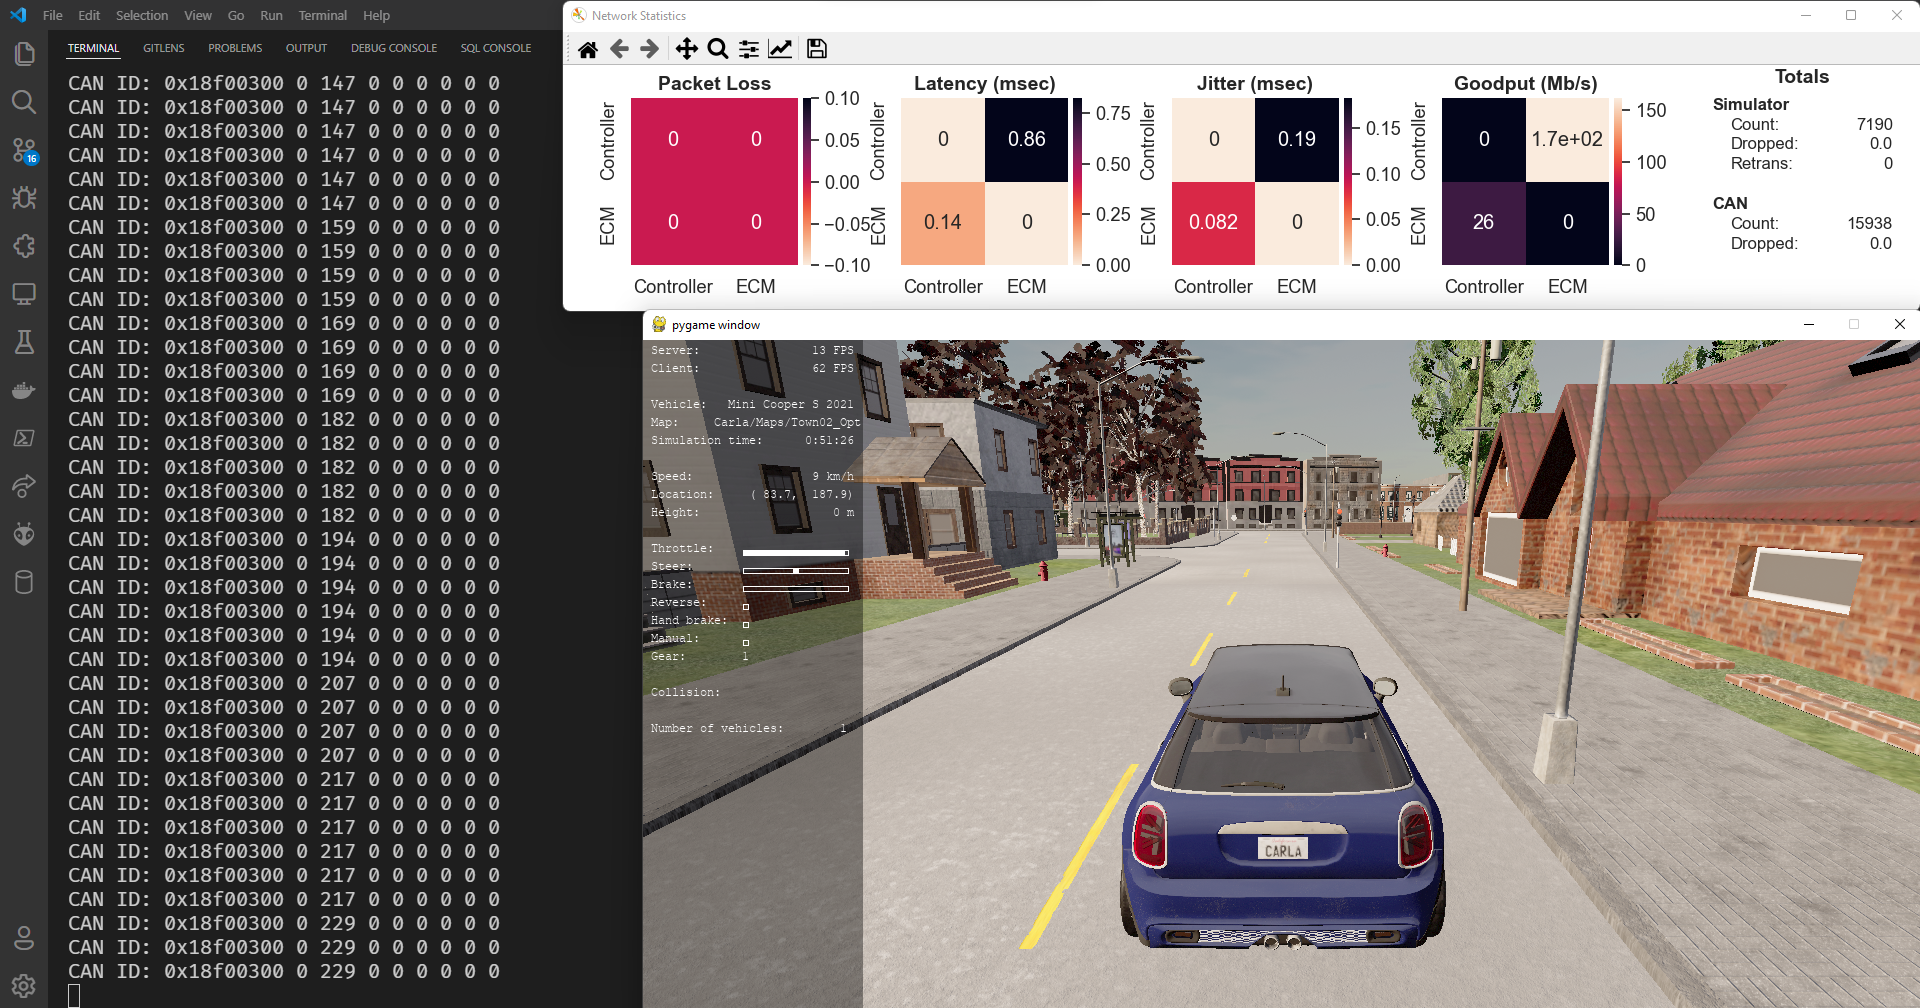
\includegraphics[width=\linewidth]{images/usability.png}
    \caption{CANLay at work in the Software Defined Truck}
    \label{fig:usabiity}
\end{figure*}
Figure \ref{fig:usabiity} shows CANLay at work. The windows in the figure display CAN frames on the left, the vehicle simulator on the bottom right, and CANLay's network health monitoring on the top right. Each of these components was already introduced in figure \ref{fig:system}. For the current purpose, we have been using the CARLA graphical vehicle simulator \cite{Dosovitskiy17}. 
Although the Carla project mainly focuses on autonomous driving research, it exposes its in-game signals through an easy-to-use python API and pays close attention to the scientific details represented in its simulator. While this is not required, the more realistic and accurate the signals are, the easier it will be to transform them into CAN messages. In this case, a specific CAN frame is printed as they are broadcasted on the overlay for this particular experiment. The ID of this frame is defined by the SAE-J1939 standards \cite{society_of_automotive_engineers_sae_nodate} and identifies engine parameters transmitted by an engine control module (ECM). The data bytes carried in the CAN frame are shown next. Of these, the second byte is shown to be changing. This particular byte carries the percentage throttle demanded by the driver. The value is also non-zero on the simulator frontend provided by the CARLA simulator.

On the top right is the network health monitoring window. It shows four matrices showing
four different metrics to estimate network health: packet loss, latency, jitter, and goodput. The significance of each of these metrics and their calculation methods were already described in the previous section. In this case, the experiment is performed over a gigabit local area network with a Layer 3 switch in between an SSSF and a Controller. Each WCANBlock wraps exactly one CAN frame. The figure shows no packets were lost while the latency in the last cycle of health report collection was less than a milliseconds between the endpoints. 
Although CANLay does not explicitly perform any latency-reducing functions, during this and other test scenarios, we noticed that the SSF and Controller forward information in the sub-milliseconds. Researchers before us have observed the same when designing CAN-to-ethernet gateways \cite{florian_polzlbauer_experience_2019}. In that light, the delay is purely due to transmission in the overlay. 
A latency of less than a millisecond is considered to be sustainable for seamless CARLA emulation at standard frame rates. 
In this particular example, the CARLA emulation frame rate was chosen to be 60 frames per second. The jitter is also fairly low in comparison to the latency. The goodput, i.e. the application data rate, is understandably higher for the ECM as it sends many more frames compared to the Controller. 


\section{Conclusion and Future Work}
In this paper, we described the concepts behind the design of CANLay, the networking backbone for the Software-Defined Truck. 
SDT is a virtualization-based experimentation framework for CAN-based security experiments and CANLay is the carrier of physical control and CAN data over long-distance networks. Essentially CANLay enables network virtualization for SDT. CAN is a reliable and low-latency network. CANLay does not explicitly ensure reliability and low latency but provides a health monitoring service that provides real-time measures of network parameters to the user. This allows the user to make critical decisions about the state of the experiment they are in.

We have identified at least three enhancements to CANLay's design that are to be pursued next. 
Firstly, we want to enable routing of actuation signals from the ECU to the vehicle simulator such that the effect ECU actuation can be visualized. We believe that the main challenge in implementing this functionality will be to enable retransmissions. Recall that at this time, CANLay piggybacks acknowledgments on CAN frames and relies on the fact that CAN frames are transmitted by the recipient ECU at a faster rate than which signals are produced by the simulator. The recipient for the actuation signals will be the Controller, but it may not transmit periodic CAN frames at a reasonably high rate. 
Secondly, we aim to enable a selective acknowledgment scheme for CAN frames. That is, enforce acknowledgment for some frames identified critical by the user, such as a frame requesting engine control in real-time. 
Finally, we aim to introduce a dynamic buffer adjustment scheme when accumulating CAN frames in a WCANBlock. This is to make optimal use of the available bandwidth while supporting high CAN busloads.

 
%-------------------------------------------------------------------------------
\bibliographystyle{plain}
\bibliography{bib}

%%%%%%%%%%%%%%%%%%%%%%%%%%%%%%%%%%%%%%%%%%%%%%%%%%%%%%%%%%%%%%%%%%%%%%%%%%%%%%%%
\end{document}
%%%%%%%%%%%%%%%%%%%%%%%%%%%%%%%%%%%%%%%%%%%%%%%%%%%%%%%%%%%%%%%%%%%%%%%%
